% Remplacement local des trois encadrés de placeholders du chapitre Homelab
% par les figures définitives ajoutées dans figures/homelab.
% Ce fichier est chargé dans un groupe LaTeX dédié afin de ne pas modifier
% le comportement de \fbox dans les chapitres suivants.
\newcounter{homelabfigureplaceholder}
\setcounter{homelabfigureplaceholder}{0}

\renewcommand{\fbox}[1]{%
  \stepcounter{homelabfigureplaceholder}%
  \ifcase\value{homelabfigureplaceholder}%
  \or
    % Figure 8.1 : architecture générale du homelab.
    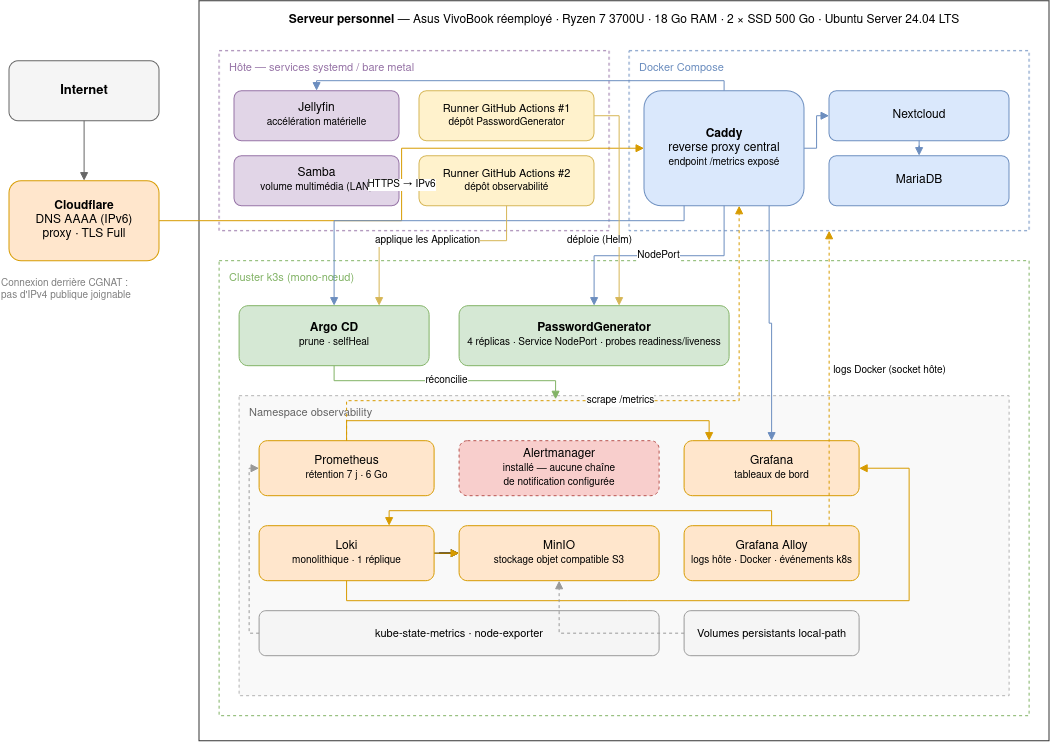
\includegraphics[width=0.96\textwidth,height=0.62\textheight,keepaspectratio]{figures/homelab/fig_8_1_architecture_homelab.png}%
  \or
    % Figure 8.2 : pipeline CI/CD de PasswordGenerator.
    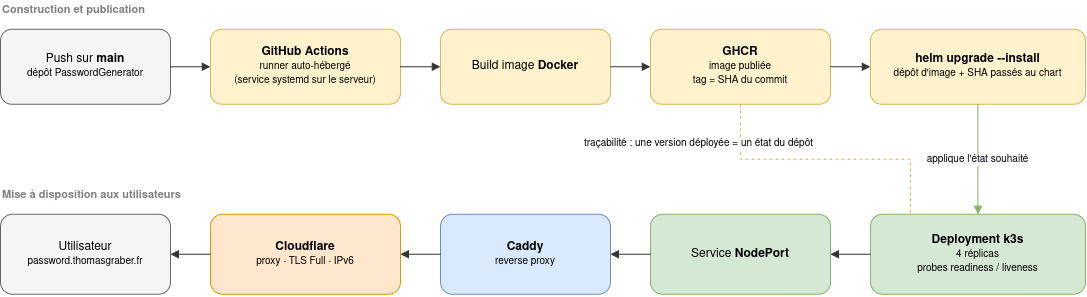
\includegraphics[width=0.96\textwidth,height=0.58\textheight,keepaspectratio]{figures/homelab/fig_8_2_pipeline_passwordgenerator.drawio.png}%
  \or
    % Figure 8.3 : comparaison des deux stratégies de déploiement.
    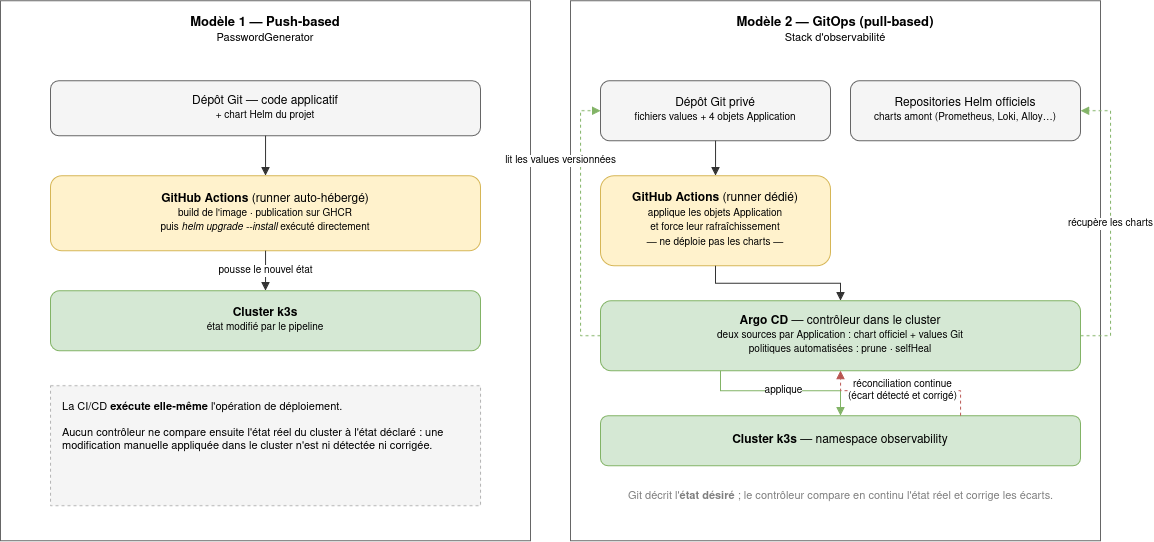
\includegraphics[width=0.96\textwidth,height=0.58\textheight,keepaspectratio]{figures/homelab/fig_8_3_deux_strategies_deploiement.drawio.png}%
  \else
    \PackageError{homelab-figures}{Nombre de placeholders Homelab inattendu}{Le chapitre Homelab contient plus de trois appels a \string\fbox.}%
  \fi
}
